% Esta es la clase que utilizamos para tomar apuntes en las asignaturas de mates y ya estoy acostumbrado a usarla. No tiene muchas cosas nuevas mas que el estilo (que podemos cambiarlo) y la cabecera y eso... Ya es el formato con el que entrego todo pero se puede usar otro si prefieres. Creo que esta basado en report (y sino en article).

\documentclass[nochap]{apuntes}

\title{Memoria Práctica 3}
\author{Víctor de Juan, Alberto Parramón, Mounaime Mellouk}
\date{C1}


% Paquetes adicionales

% --------------------
\definecolor{javared}{rgb}{0.6,0,0} % for strings
\definecolor{javagreen}{rgb}{0.25,0.5,0.35} % comments
\definecolor{javapurple}{rgb}{0.5,0,0.35} % keywords
\definecolor{javadocblue}{rgb}{0.25,0.35,0.75} % javadoc

\lstset{language=Java,
basicstyle=\ttfamily,
keywordstyle=\color{javapurple}\bfseries,
stringstyle=\color{javared},
commentstyle=\color{javagreen},
morecomment=[s][\color{javadocblue}]{/**}{*/},
numbers=left,
numberstyle=\tiny\color{black},
stepnumber=2,
numbersep=10pt,
tabsize=4,
showspaces=false,
showstringspaces=false
}

\begin{document}
\pagestyle{plain}
\maketitle

\tableofcontents
\newpage

\chapter{Detalles de la implementación}
Los detalles de implementación que son relevantes son los que vamos a comentar en las siguientes secciones, que no incluyen información sobre \textit{Regla.java}, \textit{Individuo.java}\footnote{El único detalle de esta clase es que es la que almacena la clase por defecto fija. Podría haber sido aleatoria, pero hemos preferido esta implementación} ni \textit{Poblacion.java} por su simplicidad y poca relevancia.

\section{Generación de la población inicial}

La generación de la población inicial es aleatoria, con un número de reglas por individuo fijo o variable. 

En el constructor del clasificador, se utiliza un argumento \textit{boolean numReglasAleat} que supone que el número de reglas es aleatorio (entre 1 y 2$\times$\textit{numReglas}\footnote{Parámetro recibido como argumento del constructor}) en caso de ser \textit{True} o con número de reglas fijo (e igual a \textit{numReglas}), en caso de ser \textit{False}.


\section{Cruce}
El cruce implementado es a nivel de regla. Se intercambia reglas enteras entre individuos. Se ha implementado de manera genérica de tal modo que se permite el cruce en $n$ puntos. Al ser un aspecto que consideramos menos influyente, en todas las ejecuciones han utilizado cruce en 1 punto.

En caso de que los individuos a cruzar tengan número de reglas variable, el cruce en 1 punto permite la generación de vástagos con un número de reglas distinto.

El número de reglas se determina según el punto de corte, que cada individuo tendrá un punto distinto generado aleatoriamente, entre $0$ y el número de reglas, pudiendo dar lugar a un vástago con las reglas de los 2 y al otro sin reglas.

\section{Mutación}
La mutación utilizada ha sido la propuesta en clase de teoría. 

Recorremos todos los bits de cada regla de cada individuo de la población generando un número aleatorio. Si es menor que la probabilidad de mutación de la población, entonces cambiamos el valor del bit.


\section{Selección y reemplazo}
Para ambas funcionalidades hemos utilizado el patrón de diseño \textbf{Estrategia}. Esto ha aportado una gran facilidad para intercambiar un método de selección (y de reemplazo) por otros.

\paragraph{El patrón de diseño} provoca que la clase \textit{Población.java} tenga 2 variables especiales. Una es de tipo Selección y la otra es de tipo Reemplazo. 

\begin{lstlisting}
public class Poblacion {
	...
Reemplazo estrategiaReemplazo;
Seleccion estrategiaSeleccion;
    ...
}
\end{lstlisting}

La facilidad de intercambio de método de selección (y/o de reemplazo) reside en la instanciación de una clase u otra a la hora de construir la población.

Ahora vamos a ver cada uno de los módulos: \textbf{Selección} y \textbf{Reemplazo}

\subsection{Selección}

A continuación, incluimos el diagrama de clases que hemos utilizado.

\begin{center}
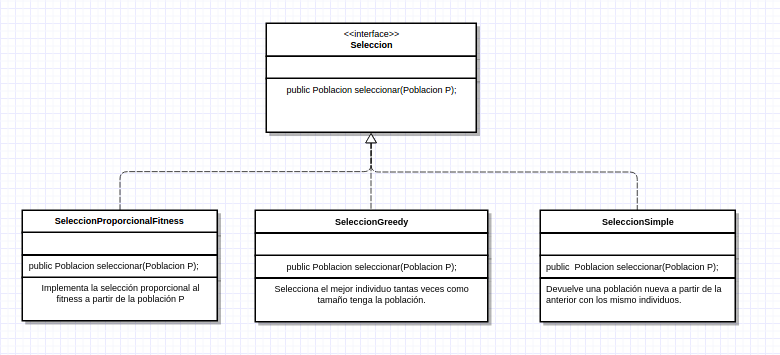
\includegraphics[scale=0.5]{img/SeleccionUML.png}
\end{center}

Hemos implementado 3 formas de selección. Cada clase simplemente implementa el método seleccionar de una manera distinta. A continuación, describimos los métodos implementados en cada clase.
\label{est:SeleccionSimple}
\begin{itemize}
 	\item \textit{SelccionSimple.java}: Implementada primera para la fase de pruebas. Es tan simple como devolver una población igual que la recibida.
 	\item \textit{SeleccionProporcionalFitness.java}: el método sugerido por el enunciado según la implementación vista en clase de teoría.
 	\item \textit{SeleccionGreedy.java} Una selección avariciosa que crea una nueva población con todos sus individuos iguales al mejor individuo de la recibida como argumento.
 \end{itemize}  


 El análisis sobre los resultados obtenidos con un método de selección u otro se encuentra en la sección de resultados (\ref{sec:Resultados}) 


\subsection{Reemplazo}
A continuación, incluimos el diagrama de clases que hemos utilizado.


\begin{center}
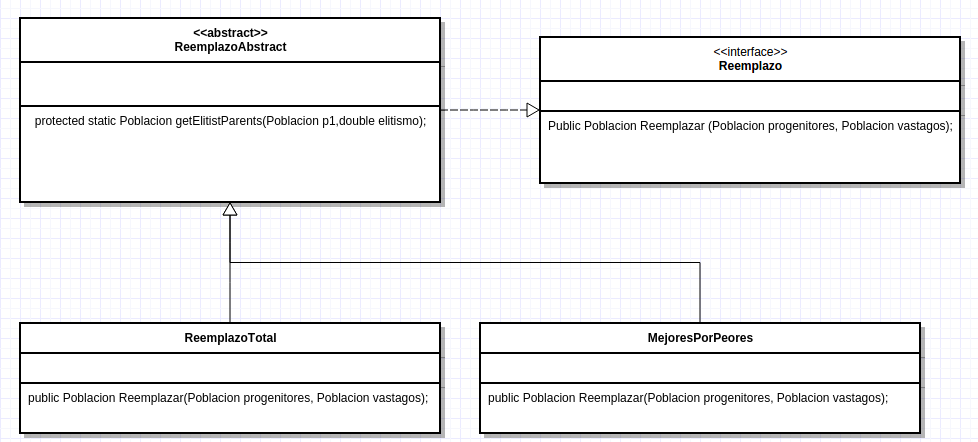
\includegraphics[scale=0.4]{img/ReemplazoUML.png}
\end{center}

La necesidad de la clase abstracta intermedia es que en la versión de Java utilizada (1.7) no es posible incluir implementaciones de métodos en una interfaz\footnote{En la siguiente versión de Java (1.8) sí es posible, pero hemos preferido utilizar la versión 1.7, creando esta clase abstracta intermedia para evitar problemas de compatibilidad}. Es por ello que incluimos la clase abstracta intermedia \textit{ReemplazoAbstract.java} con un método para seleccionar un porcentaje de la población (pensando para la selección de la élite de la población).

De esta manera, todas las maneras de reemplazar implementan de la misma manera el elitismo.

Como se aprecia en el diagrama, hemos implementado 2 clases, cada una con un método de reemplazo distinto.
\label{est:MejoresPorPeores}

\begin{itemize}
	\item \textit{ReemplazoTotal.java} implementa el reemplazo natural. Los hijos sustituyen a los padres. En caso de utilizar elitismo (sea $p$ el porcentaje de elitismo), la población resultante del reemplazo tendrá $p\%$ de padres y $(100-p)\%$ de hijos.
	\item \textit{MejoresPorPeores.java} implementa el reemplazo que pensamos que debería ser óptimo. Se juntan las 2 poblaciones (padres e hijos) y se seleccionan los $n$ mejores individuos (donde $n$ es el tamaño de la población). 
	\subitem En caso de implementar elitismo (sea $p$ el porcentaje de elitismo), la población resultante incluirá $p\%$ de padres (independientemente de que estos sean mejores que los hijos).
\end{itemize}

El análisis sobre los resultados obtenidos con un método de selección u otro se encuentra en la sección de resultados (\ref{sec:Resultados}) 


\chapter{Resultados}
\section{Tabla de resultados}

A continuación incluimos la tabla con todos los resultados obtenidos (para individuos de 11 reglas inicialmente).

\begin{center}
\begin{tabular}{cccc|c}
Reemplazo & Seleccion & Poblacion & Generaciones & Error\\\hline
ReemplazoTotal & Proporcional al Fitness & 10 & 100 & \textcolor{red}{34.769\%} \\
ReemplazoTotal & Proporcional al Fitness & 10 & 350 & 26.769\% \\
ReemplazoTotal & Proporcional al Fitness & 100 & 100 & 31.077\% \\
ReemplazoTotal & Proporcional al Fitness & 100 & 350 & 26.154\% \\
ReemplazoTotal & Proporcional al Fitness & 500 & 100 & 24.615\% \\
ReemplazoTotal & Proporcional al Fitness & 500 & 350 & \textcolor{green}{23.692\%} 
\label{tablaProfundos}
\end{tabular}
\end{center}

Vemos que el porcentaje de error se reduce al aumentar las generaciones y el tamaño de las poblaciones. Hemos tomado como máximo $350$ generaciones ya que el fitness converge rápidamente y no se produce ningún cambio, como podemos ver en las gráficas en la sección \ref{sec:evolucionFitness}.

Como era de esperar, con un mayor tamaño de población y más generaciones obtenemos porcentajes mejores. Aunque estos porcentajes de error son demasiado altos como para poder utilizar este algoritmo en un entorno real de producción.

Por otro lado, al aumentar el tamaño de la población, el número de generaciones no influye mucho. Es por ello también que decidimos reducir el tamaño máximo de la población a 350 (en vez de 100 como sugería el enunciado.)

\section{Análisis de resultados}
\label{sec:Resultados}

\subsection{Estrategias de reemplazo y selección}

Hemos incluido en esta subsección una comparativa de los rendimientos de cada una de las estrategias de selección y de reemplazo. A continuación, mostramos la tabla con los resultados, para 73 generaciones y poblaciones de 73 individuos.\footnote{La selección de este número ha sido arbitraria, buscando un número no demasiado grande por los tiempo de ejecución pero suficientemente grande para que se pudieran apreciar diferencias.}


\begin{center}
\begin{tabular}{cccc|c}
Reemplazo & Seleccion   & Error\\\hline
ReemplazoTotal & SeleccionProporcionalAlFitness & 26.769\% \\
ReemplazoTotal & SeleccionAvariciosa & 29.846\% \\
ReemplazoTotal & SeleccionSimple & 31.692\% \\
MejoresPorPeores & SeleccionProporcionalAlFitness & 31.385\% \\
MejoresPorPeores & SeleccionAvariciosa & 31.077\% \\
MejoresPorPeores & SeleccionSimple & \textcolor{green}{26.154}\% \\
\end{tabular}
\end{center}

Vemos que la mejor combinación es la estrategia de reemplazo ``Mejores por peores'' (\ref{est:MejoresPorPeores}) con la selección simple (\ref{est:SeleccionSimple}), aunque esta diferencia no parece muy significativa.

Nos hubiera gustado poder comparar todas las estrategias de selección y de reemplazo con los parámetros sugeridos por el enunciado, pero esto no ha sido posible debido al excesivo tiempo de dicha ejecución. \footnote{La tuvimos que suspender después de 30 horas en funcionamiento}

\subsection{Importancia del número de Reglas}
\label{subsec:numReglas}

El número de reglas es un factor muy importante. Si tenemos una única regla, será muy poco probable que los datos a clasificar la cumplan y por lo tanto asignaremos la clase por defecto a prácticamente todos los datos, provocando una clasificación muy sesgada. En caso de tener demasiadas reglas a las que asignamos una clase, es fácil que los datos a clasificar cumplan alguna de esas reglas (por las disyuntivas de las reglas). Por otro lado, al tener muchas reglas, hay más posibilidades de que se generen a partir de mutaciones y cruces las reglas óptimas.

Por ello, hemos tomado 2 decisiones. La primera es el estudio de la importancia del número de regla, utilizando un número fijo de reglas para todos los individuos. Además, el número de reglas utilizado en el análisis de los resultados ha sido variable,  dando lugar a una mejor algoritmo de esta manera.

A continuación, la tabla de los resultados del estudio de la importancia del número de reglas.

\begin{center}
\begin{tabular}{cc}
Reglas&Error\\\hline
5 & 29.846\%\\
11 & 22.462\%\\
16 & 31.077\%\\
25 & 27.692\%\\
50 & 68.923\%\\
150 & 64.615\%\\
\end{tabular}
\end{center}
Los par\'amemtros utilizados han sido:\begin{itemize}
\item \#Individuos: 75 \item Generaciones: 75 \item Elitismo: 5.00\%\item PCruce: 60.00\%\item PMut: 1.00\%\item Reemplazo: SeleccionProporcionalAl\item Selecci\'on: MejoresPorPeores
\end{itemize}


Vemos que es un factor influyente. Por estos resultados es por los que hemos elegido un número inicial de reglas = 11 (aunque lo que sugería el enunciado era cercano a 25).


\section{Evolución del fitness}

\label{sec:evolucionFitness}

\subsection{Ejecuciones de la tabla de resultados}
Estas gráficas corresponden a las ejecuciones de la tabla con los porcentajes de error(\ref{tablaProfundos}). Recordamos los parámetros:

\begin{itemize}
	\item \textbf{Selección:} Proporcional al fitess.
	\item \textbf{Reemplazo:} Reemplazo total.
	\item \textbf{Número de reglas:} Número inicial 11 reglas, pero es una cantidad variable.
\end{itemize}


\paragraph{Evolución del fitness para 350 generaciones y poblaciones de 10 individuos}
\begin{center}
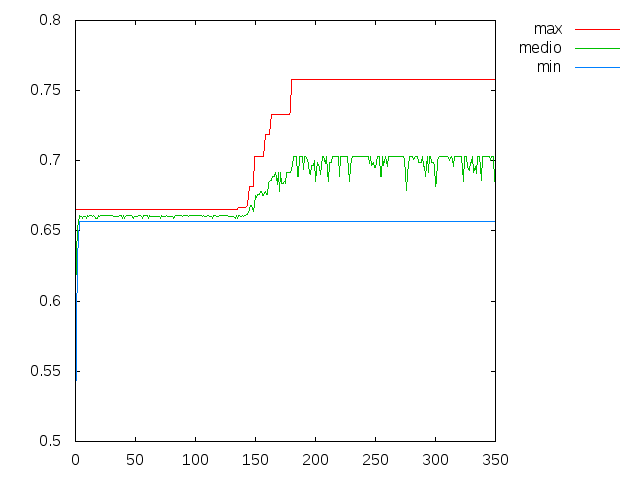
\includegraphics[scale=0.6]{tex/img/g350_p10_ReemplazoTotal_SeleccionProporcionalAlFitness_reg11.png}
\end{center}
\paragraph{Evolución del fitness para 350 generaciones y poblaciones de 100 individuos}
\begin{center}
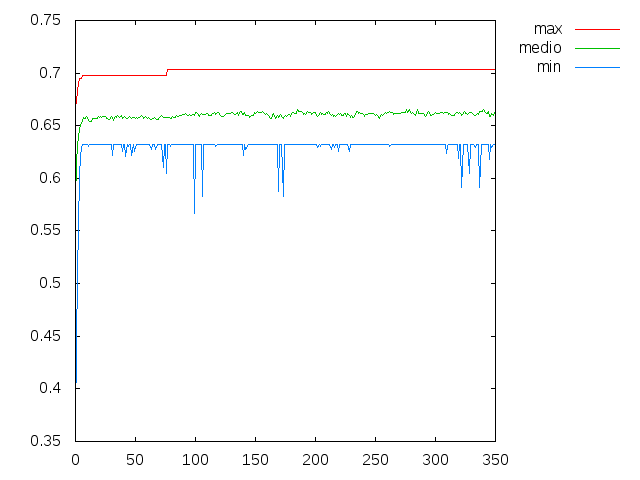
\includegraphics[scale=0.6]{tex/img/g350_p100_ReemplazoTotal_SeleccionProporcionalAlFitness_reg11.png}
\end{center}
\paragraph{Evolución del fitness para 350 generaciones y poblaciones de 500 individuos}
\begin{center}
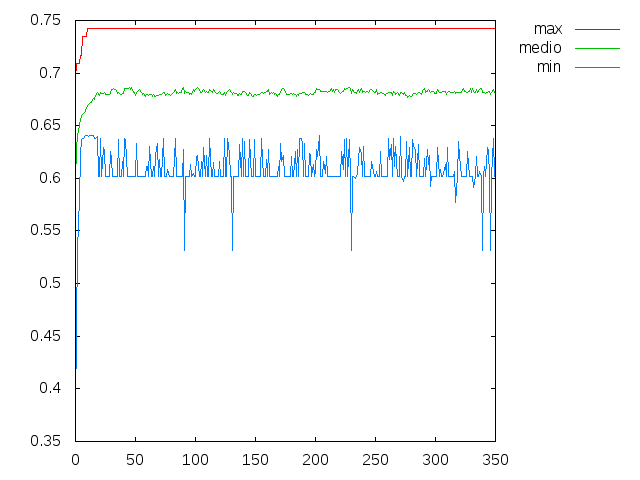
\includegraphics[scale=0.6]{tex/img/g350_p500_ReemplazoTotal_SeleccionProporcionalAlFitness_reg11.png}
\end{center}

\paragraph{Evolución del fitness para 100 generaciones y poblaciones de 10 individuos}
\begin{center}
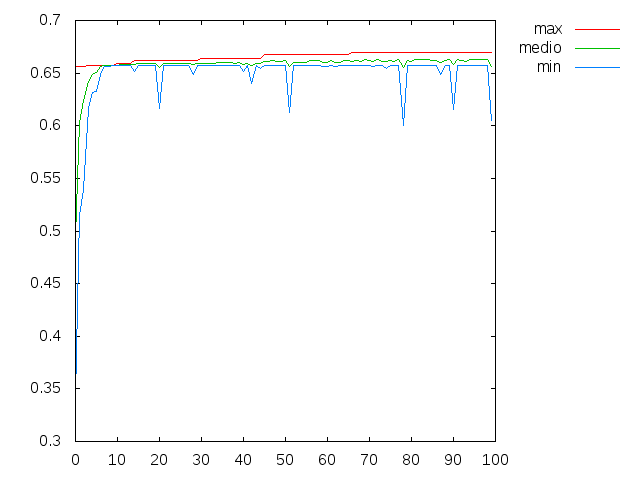
\includegraphics[scale=0.6]{tex/img/g100_p10_ReemplazoTotal_SeleccionProporcionalAlFitness_reg11.png}
\end{center}
\paragraph{Evolución del fitness para 100 generaciones y poblaciones de 100 individuos}
\begin{center}
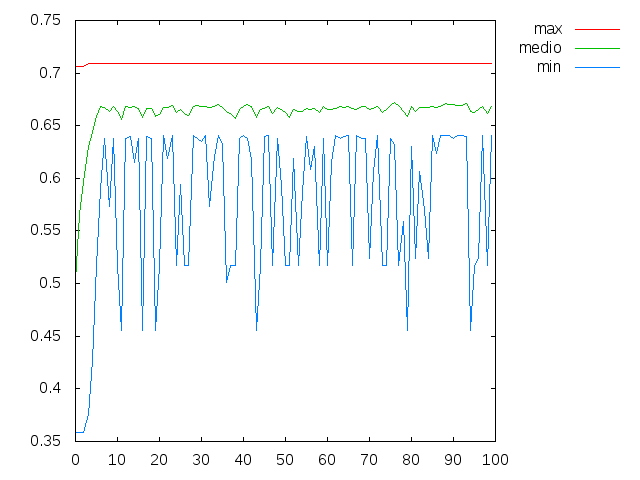
\includegraphics[scale=0.6]{tex/img/g100_p100_ReemplazoTotal_SeleccionProporcionalAlFitness_reg11.png}
\end{center}
\paragraph{Evolución del fitness para 100 generaciones y poblaciones de 500 individuos}
\begin{center}
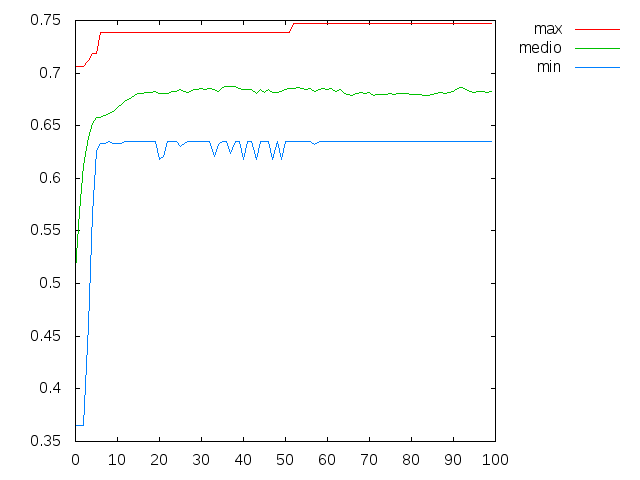
\includegraphics[scale=0.6]{tex/img/g100_p500_ReemplazoTotal_SeleccionProporcionalAlFitness_reg11.png}
\end{center}


\subsection{Comparativa de estrategias de selección y reemplazo}

Todas estas gráficas han sido generadas para 73 generaciones y poblaciones de 73 individuos. Primero mostramos las gráficas y a continuación un breve análisis.



\paragraph{Reemplazo total, Selección Proporcional}
\begin{center}
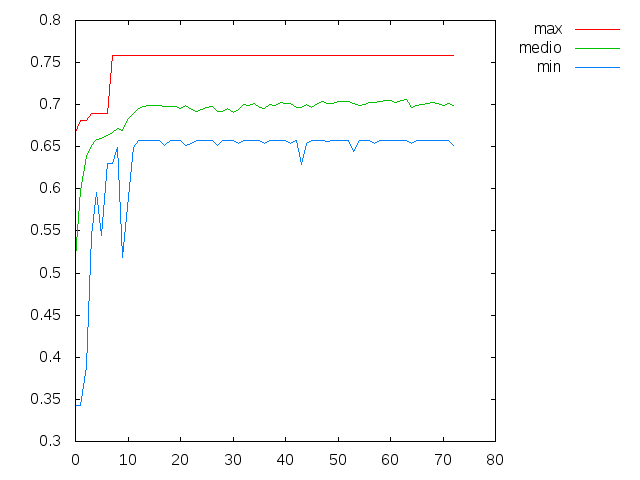
\includegraphics[scale=0.6]{tex/img/g73_p73_ReemplazoTotal_SeleccionProporcionalAlFitness_reg11.png}
\end{center}

\paragraph{Reemplazo total, Selección Simple}
\begin{center}
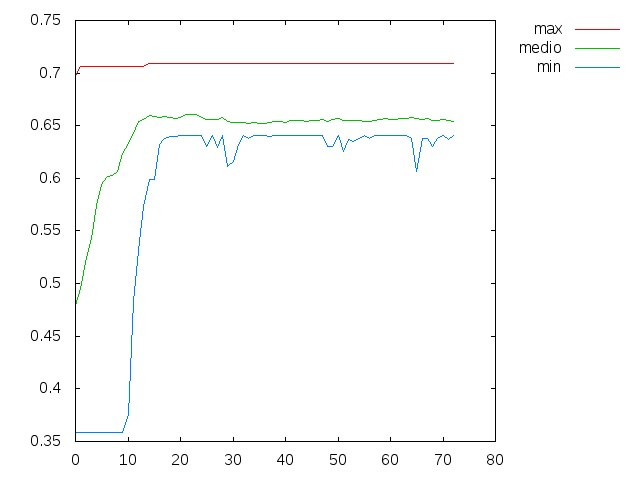
\includegraphics[scale=0.6]{tex/img/g73_p73_ReemplazoTotal_SeleccionSimple_reg11.png}
\end{center}

\paragraph{Reemplazo total, Selección Avariciosa}
\begin{center}
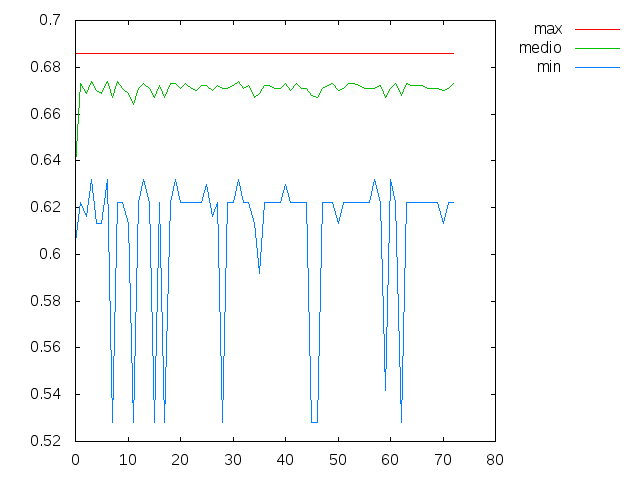
\includegraphics[scale=0.6]{tex/img/g73_p73_ReemplazoTotal_SeleccionAvariciosa_reg11.png}
\end{center}

\paragraph{Mejores por Peores, Selección Proporcional}
\begin{center}
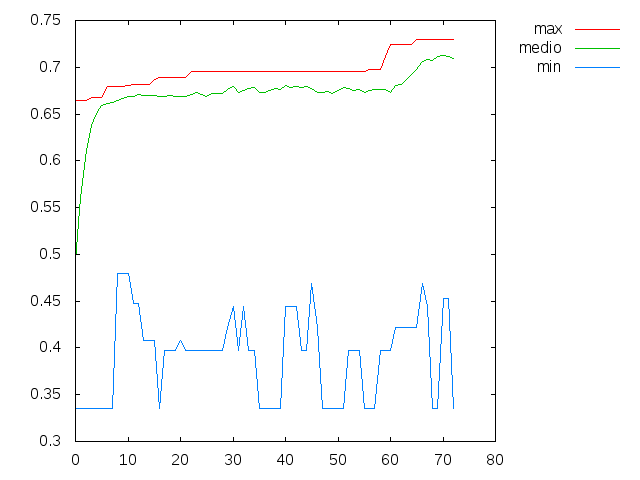
\includegraphics[scale=0.6]{tex/img/g73_p73_MejoresPorPeores_SeleccionProporcionalAlFitness_reg11.png}
\end{center}

\paragraph{Mejores por Peores, Selección Simple}
\begin{center}
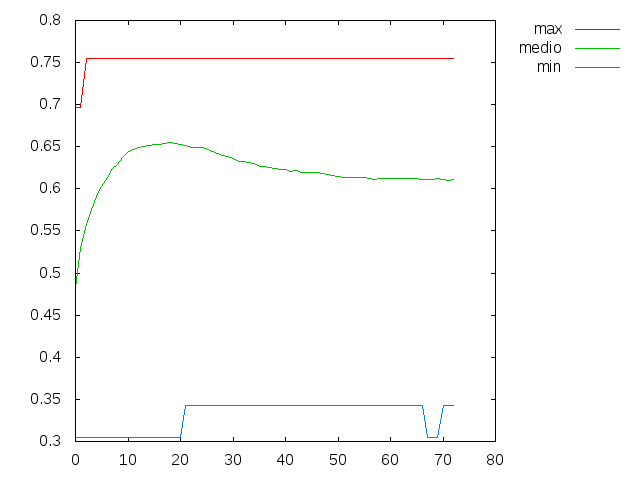
\includegraphics[scale=0.6]{tex/img/g73_p73_MejoresPorPeores_SeleccionSimple_reg11.png}
\end{center}

Es curiosa la gráfica generada por el fitness medio de estas poblaciones. Esto tal vez es lo que `` Sir Francis Galton'' definió como \textbf{regresión a la mediocridad}. 


\paragraph{Mejores por Peores, Selección Avariciosa}
\begin{center}
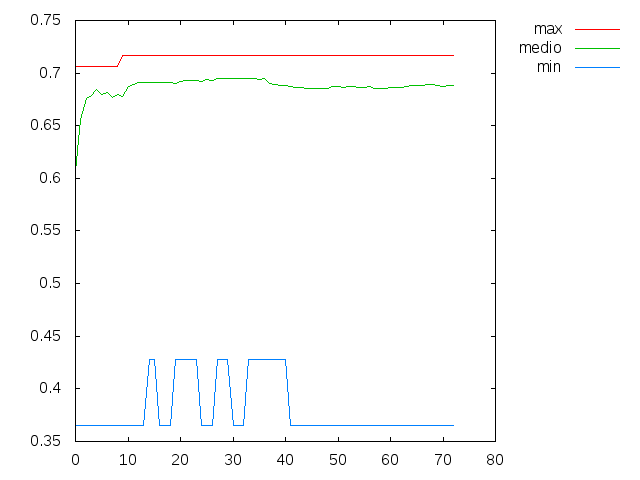
\includegraphics[scale=0.6]{tex/img/g73_p73_MejoresPorPeores_SeleccionAvariciosa_reg11.png}
\end{center}

Se puede observar cómo los fitness medios de la estrategia de reemplazo ``Mejores por Peores'' son más cercanos a los  fitness máximos. Por otro, vemos que los fitness mínimos del reemplazo total son mayores. 

La explicación de tener unos fitness mínimos menores y un fitness medio más alto se debe a la cantidad de individuos con buen fitness. Al seleccionar los mejores de las 2 poblaciones (vástagos y progenitores), obtenemos, en media, fitness mayores, aunque pueda haber algún individuo con un fitness extremadamente bajo. 

Por último, comentamos los valores máximos de fitness alcanzados. Esperábamos que el fitness máximo de la selección avariciosa, con un reemplazo de ``Mejores por peores'' fuera la más alta, pero esta aproximación es demasiado ingenua. El fitness máximo se alcanza utilizando el reemplazo total y la selección proporcional al fitness.\footnote{Es 0.03 mayor que el fitness de la selección simple con la estrategia de reemplazo ``Mejores por peores''}. 



\appendix


\chapter{Evolución del fitness para número de reglas fijo}

Primero mostramos las gráficas y a continuación un breve análisis.
\paragraph{Evolución del fitness para un número fijo de $5$ reglas}
\begin{center}
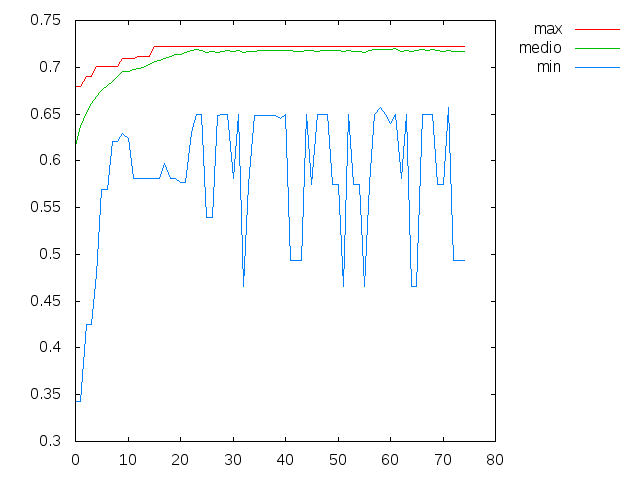
\includegraphics[scale=0.6]{tex/img/g75_p75_MejoresPorPeores_SeleccionProporcionalAlFitness_reg5.png}
\end{center}
\paragraph{Evolución del fitness para un número fijo de $11$ reglas}
\begin{center}
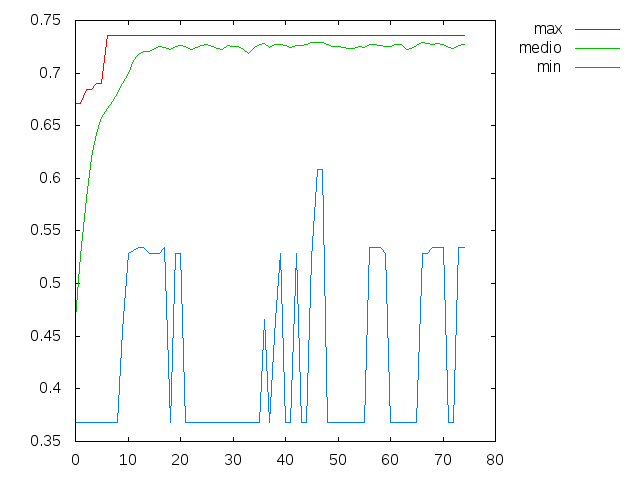
\includegraphics[scale=0.6]{tex/img/g75_p75_MejoresPorPeores_SeleccionProporcionalAlFitness_reg11.png}
\end{center}
\paragraph{Evolución del fitness para un número fijo de $16$ reglas}
\begin{center}
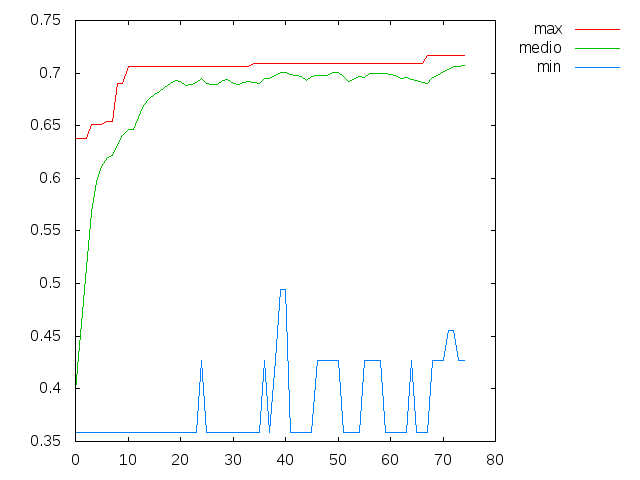
\includegraphics[scale=0.6]{tex/img/g75_p75_MejoresPorPeores_SeleccionProporcionalAlFitness_reg16.png}
\end{center}
\paragraph{Evolución del fitness para un número fijo de $25$ reglas}
\begin{center}
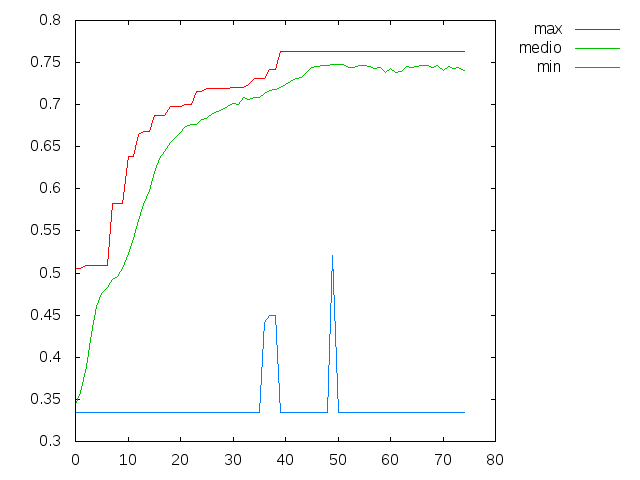
\includegraphics[scale=0.6]{tex/img/g75_p75_MejoresPorPeores_SeleccionProporcionalAlFitness_reg25.png}
\end{center}
\paragraph{Evolución del fitness para un número fijo de $50$ reglas}
\begin{center}
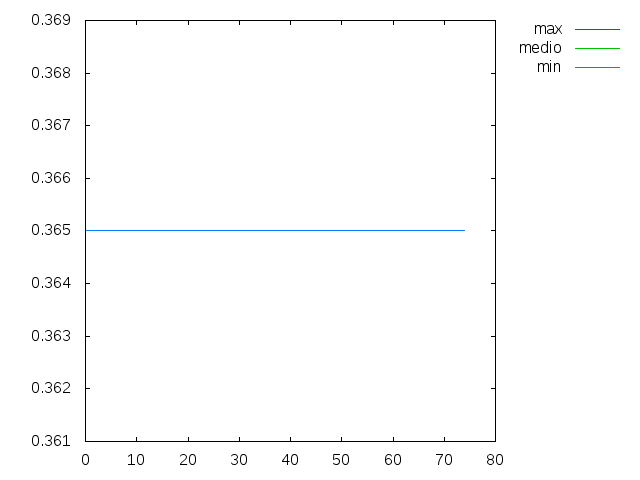
\includegraphics[scale=0.6]{tex/img/g75_p75_MejoresPorPeores_SeleccionProporcionalAlFitness_reg50.png}
\end{center}
\paragraph{Evolución del fitness para un número fijo de $150$ reglas}
\begin{center}
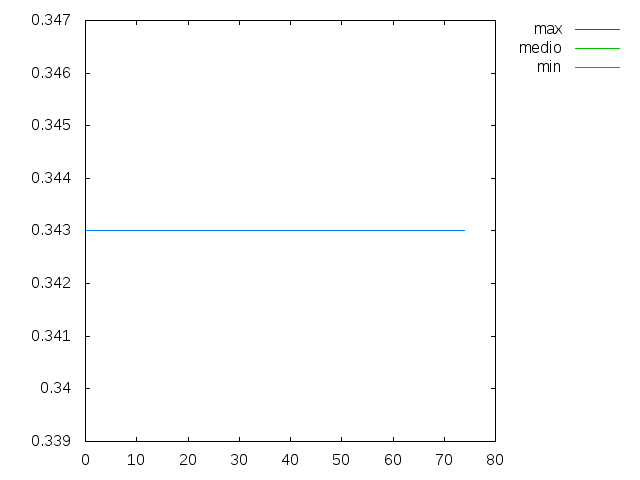
\includegraphics[scale=0.6]{tex/img/g75_p75_MejoresPorPeores_SeleccionProporcionalAlFitness_reg150.png}
\end{center}

Se puede ver cómo el fitness medio (en verde) es más cercano al máximo cuantas menos reglas tenemos. Esto se debe a que el fitness mínimo es, en general, mayor cuantas menos reglas tienen los individuos. Pero lo más interesante de ver es cómo para 25 reglas, la convergencia es mucho más lenta, empieza en un valor mucho menor, con un fitness medio muy cercano al mínimo, para al final acabar llegando a valores similares.

Por otro lado, al aumentar demasiado el número de reglas (y mantenerlo fijo), el fitness mínimo, medio y máximo se mantienen constantes para todas las generaciones.

Por último, si observamos los valores máximos alcanzados, con $25$ reglas se obtiene un fitness mayor.


\chapter{Evolución gráfica del número de reglas}
\section{Ejemplo 1}
A continuación, mostramos la evolución del fitness y el número de reglas (del mejor individuo) para cada población.

\begin{center}
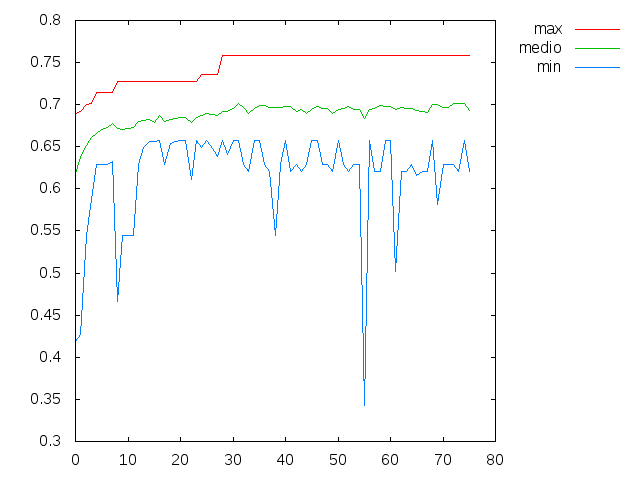
\includegraphics[scale=0.4]{tex/img/g76_p76_ReemplazoTotal_SeleccionProporcionalAlFitness_reg11.png}
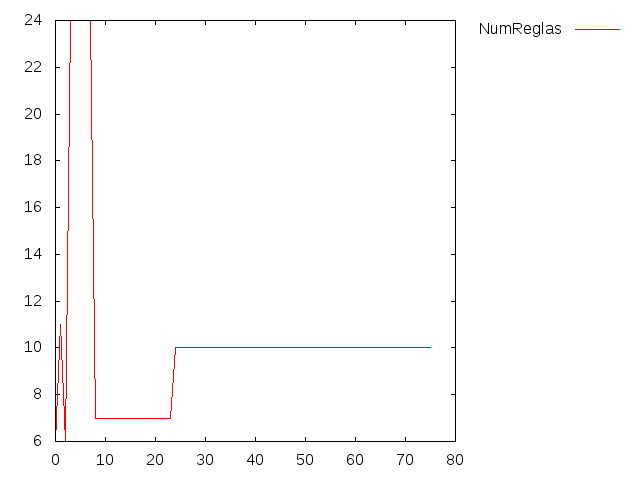
\includegraphics[scale=0.4]{tex/img/g76_p76_ReemplazoTotal_SeleccionProporcionalAlFitness_reg11_reglas.png}
\end{center}

Vemos que obtenemos un fitness parecido a las 25 reglas anteriores, pero con una convergencia mayor. El valor constante final es $10$, lo que es perfectamente coherente con el análisis de la importancia del número de reglas.


\section{Ejemplo 2}
A continuación incluimos otro ejemplo ilustrativo, en el que comparamos la evolución del número de reglas y del fitness en 2 casos distintos.


\paragraph{Evolución de reglas y fitness} para la ejecución con 73 individuos y 73 generaciones utilizando la selección proporcional a fitness y el reemplazo ``Mejores por peores''.

\begin{center}
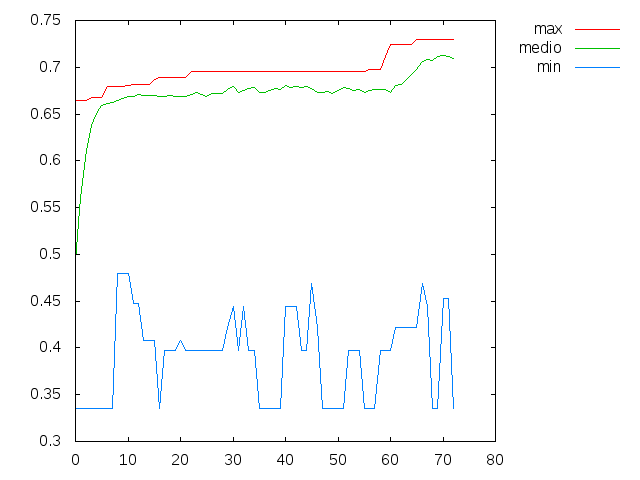
\includegraphics[scale=0.4]{tex/img/g73_p73_MejoresPorPeores_SeleccionProporcionalAlFitness_reg11.png}
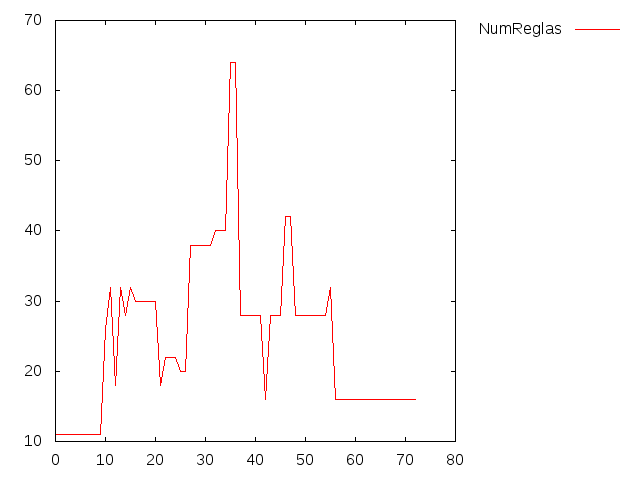
\includegraphics[scale=0.4]{tex/img/g73_p73_MejoresPorPeores_SeleccionProporcionalAlFitness_reg11_reglas.png}
\end{center}

\paragraph{Evolución de reglas y fitness} para la ejecución con 73 individuos y 73 generaciones utilizando la selección proporcional a fitness y el reemplazo ``Reemplazo Total''.
\begin{center}
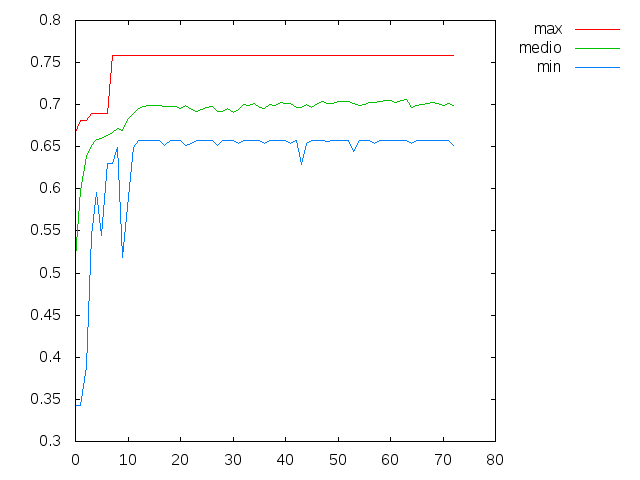
\includegraphics[scale=0.4]{tex/img/g73_p73_ReemplazoTotal_SeleccionProporcionalAlFitness_reg11.png}
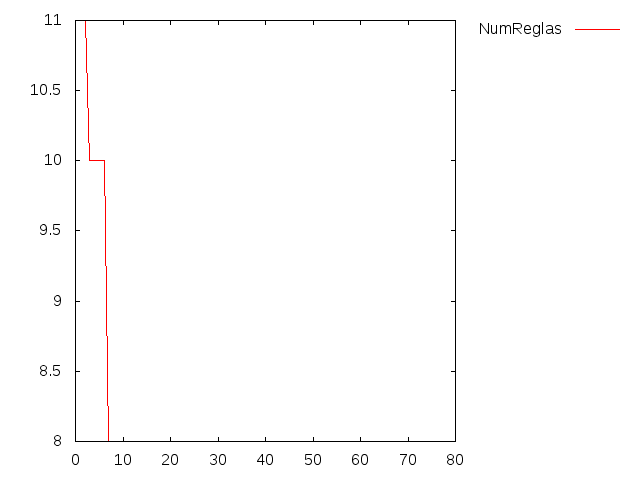
\includegraphics[scale=0.4]{tex/img/g73_p73_ReemplazoTotal_SeleccionProporcionalAlFitness_reg11_reglas.png}
\end{center}

Ambos números de reglas iniciales son 11, y en ambas gráficas vemos que se estabiliza, manteniéndose constante. Con la estrategia de ``Reemplazo total'', se estabiliza en 8 reglas, mientras que ``Mejores por peores'' se estabiliza en 16.

Esto confirma que la elección de $11$ reglas iniciales es una buena elección.


\end{document}
